\documentclass[border=10pt]{standalone}
\usepackage[svgnames]{xcolor}
\usepackage{amsmath}
\usepackage{pgfplots}
\pgfplotsset{compat=newest}
\usepackage[sfdefault]{FiraSans}
\usepackage{FiraMono}
\renewcommand*\familydefault{\sfdefault}
\begin{document}
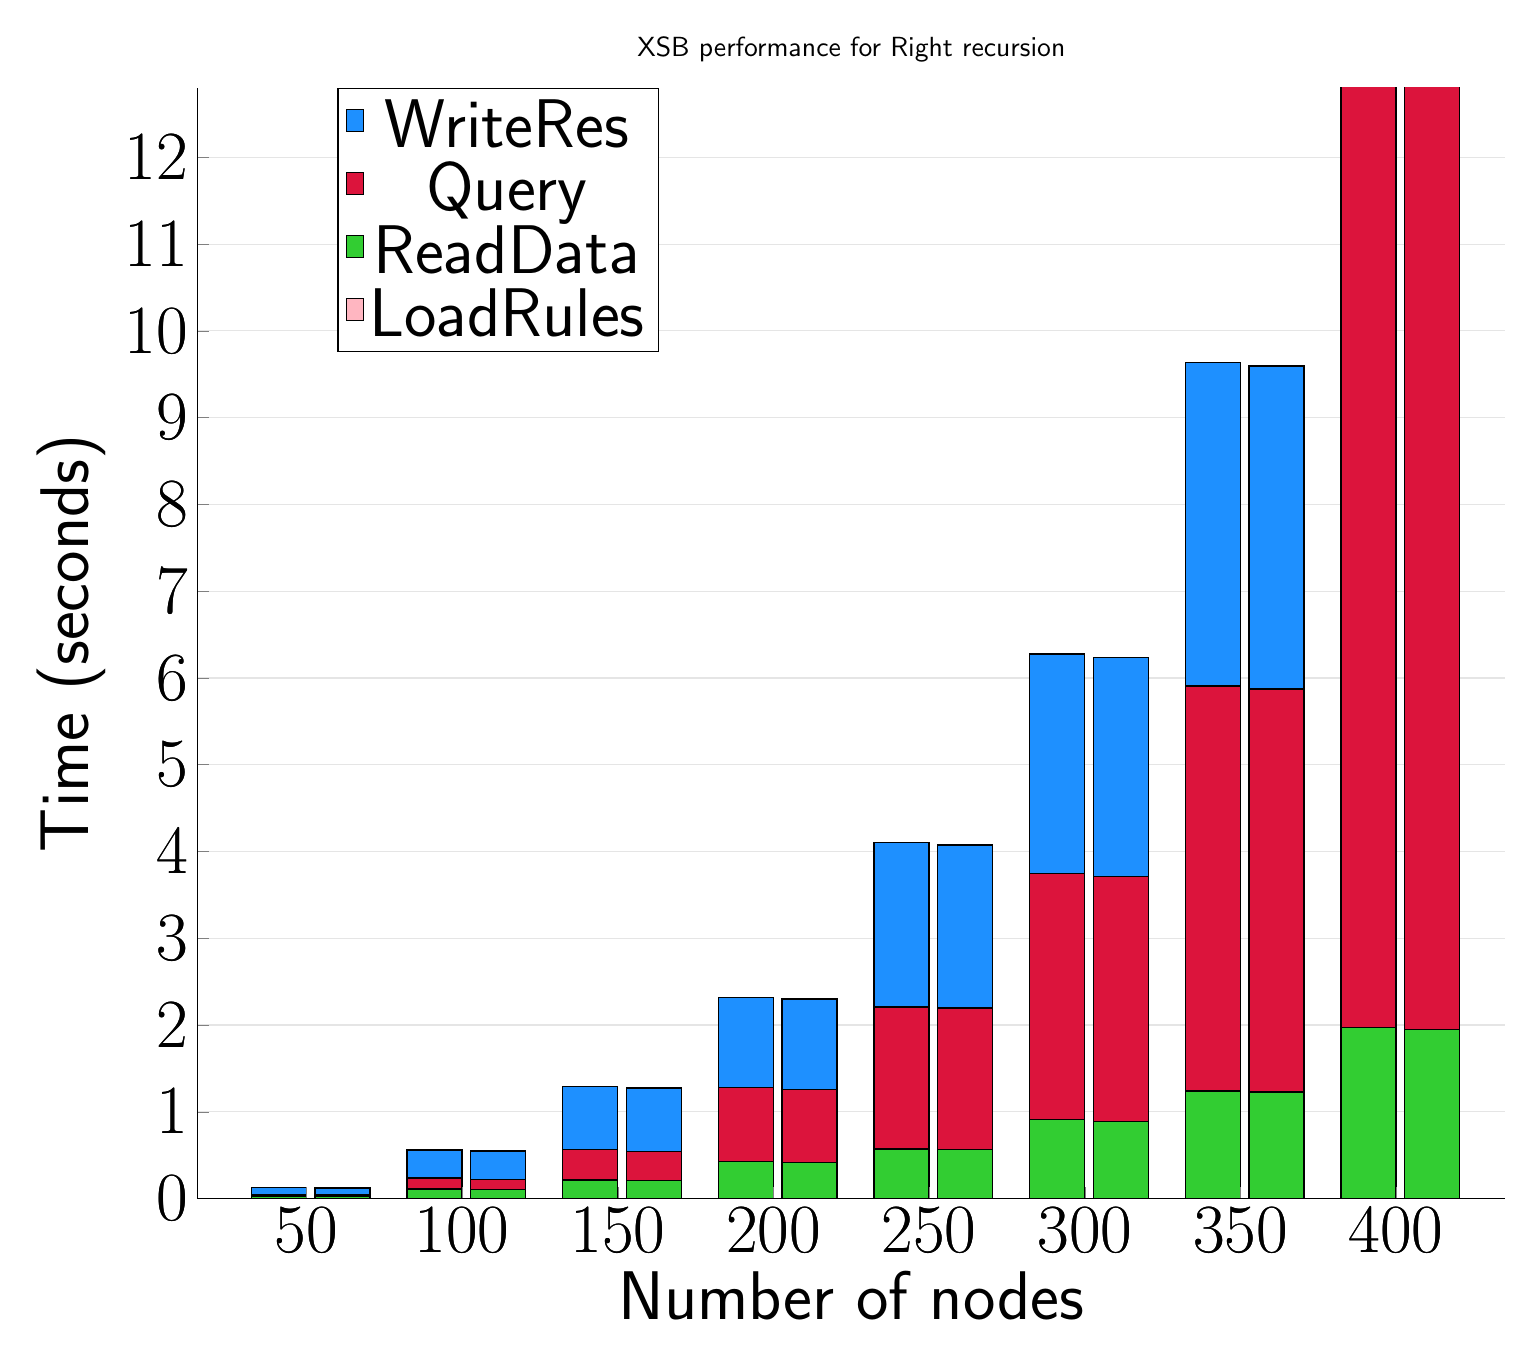
\begin{tikzpicture}
\begin{axis}[
   ybar stacked,
   title={XSB performance for Right recursion},
   bar shift=-10pt,
   width=1.5\textwidth,
   bar width=0.7cm,
   ymajorgrids, tick align=inside,
   major grid style={draw=gray!20},
   xtick=data,
   ymin=0, ymax=12.800821224848427,
   axis x line*=bottom,
   axis y line*=left,
   enlarge x limits=0.1,
   legend style={
       at={(0.23, 1)},
       anchor=north,
       legend columns=1,
       font=\Huge,
   },
   ylabel={Time (seconds)},
   xlabel={Number of nodes},
   label style={font=\Huge},
   tick label style={font=\Huge},
]
\addlegendimage{fill=DodgerBlue, draw=black, line width=0.2pt}
\addlegendentry{WriteRes}
\addlegendimage{fill=Crimson, draw=black, line width=0.2pt}
\addlegendentry{Query}
\addlegendimage{fill=LimeGreen, draw=black, line width=0.2pt}
\addlegendentry{ReadData}
\addlegendimage{fill=LightPink, draw=black, line width=0.2pt}
\addlegendentry{LoadRules}
\addplot +[fill=LightPink, draw=black, line width=0.5pt] coordinates {
    (50, 0.003561019897460937)
    (100, 0.004222393035888674)
    (150, 0.00305032730102539)
    (200, 0.0034348964691162096)
    (250, 0.003172953923543293)
    (300, 0.003332614898681643)
    (350, 0.00318169593811035)
    (400, 0.003760894139607743)
};
\addplot +[fill=LimeGreen, draw=black, line width=0.5pt] coordinates {
    (50, 0.027437766393025698)
    (100, 0.10812664031982407)
    (150, 0.21093575159708666)
    (200, 0.42276334762573237)
    (250, 0.566895008087158)
    (300, 0.905372381210327)
    (350, 1.2377160390218134)
    (400, 1.9689037799835198)
};
\addplot +[fill=Crimson, draw=black, line width=0.5pt] coordinates {
    (50, 0.015837272008260097)
    (100, 0.12493101755778001)
    (150, 0.350019613901774)
    (200, 0.8516953786214193)
    (250, 1.6362059116363499)
    (300, 2.8366053104400635)
    (350, 4.6660923163096095)
    (400, 13.500138680140166)
};
\addplot +[fill=DodgerBlue, draw=black, line width=0.5pt] coordinates {
    (50, 0.07831931114196783)
    (100, 0.32327397664388036)
    (150, 0.7294730345408126)
    (200, 1.042235294977824)
    (250, 1.899861494700117)
    (300, 2.530195077260337)
    (350, 3.7300600210825596)
    (400, 2.3969443639119334)
};
\end{axis}
\begin{axis}[
   ybar stacked,
   bar shift=13pt,
   width=1.5\textwidth,
   bar width=0.7cm,
   ymajorgrids, tick align=inside,
   major grid style={draw=none},
   xtick=data,
   ymin=0, ymax=12.800821224848427,
   axis x line*=none,
   axis y line*=none,
   enlarge x limits=0.1,
   label style={font=\Huge},
   tick label style={font=\Huge},
]
\addplot +[fill=LightPink, draw=black, line width=0.5pt] coordinates {
    (50, 0.003408666666666667)
    (100, 0.00420033333333333)
    (150, 0.0030189999999999995)
    (200, 0.0028553333333333334)
    (250, 0.0031286666666666667)
    (300, 0.0033333333333333335)
    (350, 0.0031806666666666667)
    (400, 0.00336566666666667)
};
\addplot +[fill=LimeGreen, draw=black, line width=0.5pt] coordinates {
    (50, 0.027361999999999997)
    (100, 0.09817133333333333)
    (150, 0.20490966666666666)
    (200, 0.41593233333333335)
    (250, 0.5655023333333333)
    (300, 0.8820236666666667)
    (350, 1.2247656666666666)
    (400, 1.9457556666666669)
};
\addplot +[fill=Crimson, draw=black, line width=0.5pt] coordinates {
    (50, 0.015841333333333332)
    (100, 0.11494733333333333)
    (150, 0.3373923333333333)
    (200, 0.8351596666666666)
    (250, 1.6271713333333333)
    (300, 2.8277180000000004)
    (350, 4.644032333333333)
    (400, 13.368732333333334)
};
\addplot +[fill=DodgerBlue, draw=black, line width=0.5pt] coordinates {
    (50, 0.07406533333333333)
    (100, 0.32948133333333335)
    (150, 0.728805)
    (200, 1.046429)
    (250, 1.8803869999999998)
    (300, 2.5208250000000003)
    (350, 3.723563)
    (400, 2.193531)
};
\end{axis}
\end{tikzpicture}

\end{document}
